\section*{Domácí úloha 2}

\subsection*{Příklad č.~6}

Najděte všechny podgrupy $(\mathbb{Z}_{6}, \oplus)$. Které z nich jsou normální? Sestrojte příslušné faktorové grupy.

\begin{eqnarray*}
\mathbb{Z}_{6} &=& \lbrace 0, 1, 2, 3, 4, 5 \rbrace \\
a \oplus b &=& (a + b) \mod 6
\end{eqnarray*}

\minipage{0.50\textwidth}
\begin{center}
\begin{tabular}{|c|c|c|c|c|c|c|}
\hline
$\oplus$ & 0 & 1 & 2 & 3 & 4 & 5\\
\hline
0        & 0 & 1 & 2 & 3 & 4 & 5 \\
\hline
1        & 1 & 2 & 3 & 4 & 5 & 0 \\
\hline
2        & 2 & 3 & 4 & 5 & 0 & 1 \\
\hline
3        & 3 & 4 & 5 & 0 & 1 & 2 \\
\hline
4        & 4 & 5 & 0 & 1 & 2 & 3 \\
\hline
5        & 5 & 0 & 1 & 2 & 3 & 4 \\
\hline
\end{tabular}
\end{center}
\endminipage
\minipage{0.50\textwidth}
\begin{itemize}
\item Jednotkový prvek je $0$.
\item Inverzní prvek $a \oplus a^{-1} = 0$.
\end{itemize}
$
\left.{\begin{array}{l}
0 \oplus 0 = 0 \\
0 \oplus 1 = 1 \\
0 \oplus 2 = 2 \\
0 \oplus 3 = 3 \\
0 \oplus 4 = 4 \\
0 \oplus 5 = 5 \\
\end{array}}\right\} = \mathbb{Z}_{6}
$
\endminipage

\minipage{0.16\textwidth}
\begin{eqnarray*}
0 \oplus 0 &=& 0
\end{eqnarray*}
\endminipage
\minipage{0.16\textwidth}
\begin{eqnarray*}
0 \oplus 1 &=& 1 \\
1 \oplus 1 &=& 2 \\
2 \oplus 1 &=& 3 \\
3 \oplus 1 &=& 4 \\
4 \oplus 1 &=& 5 \\
5 \oplus 1 &=& 0
\end{eqnarray*}
\endminipage
\minipage{0.16\textwidth}
\begin{eqnarray*}
0 \oplus 2 &=& 2 \\
2 \oplus 2 &=& 4 \\
4 \oplus 2 &=& 0
\end{eqnarray*}
\endminipage
\minipage{0.16\textwidth}
\begin{eqnarray*}
0 \oplus 3 &=& 3 \\
3 \oplus 3 &=& 0
\end{eqnarray*}
\endminipage
\minipage{0.16\textwidth}
\begin{eqnarray*}
0 \oplus 4 &=& 4 \\
4 \oplus 4 &=& 2 \\
2 \oplus 4 &=& 0
\end{eqnarray*}
\endminipage
\minipage{0.16\textwidth}
\begin{eqnarray*}
0 \oplus 5 &=& 5 \\
1 \oplus 5 &=& 0 \\
2 \oplus 5 &=& 1 \\
3 \oplus 5 &=& 2 \\
4 \oplus 5 &=& 3 \\
5 \oplus 5 &=& 4
\end{eqnarray*}
\endminipage

\minipage{0.5\textwidth}
\begin{eqnarray*}
T_{1} &=& \lbrace 0 \rbrace \\
T_{2} &=& \mathbb{Z}_{6} = \\ &=& \lbrace 0, 1, 2, 3, 4, 5 \rbrace \\
T_{3} &=& \lbrace 0, 2, 4 \rbrace \\
T_{4} &=& \lbrace 0, 3 \rbrace \\
T_{5} &=& T_{3} \\
T_{6} &=& T_{2}
\end{eqnarray*}
\endminipage
\minipage{0.5\textwidth}
\begin{eqnarray*}
n &\in& N \\
0 \oplus n &\rightarrow& 0 \\
1 \oplus n &\rightarrow& T_{2}
\end{eqnarray*}
Pokud vybereme dva prvky ze stejné cyklické grupy, tak vyjde něco, co bude patřit dané grupě.
\endminipage

\minipage{0.5\textwidth}
$2,3$ \\
$2$ vygeneruje $0,2,4$ \\
$3$ vygeneruje $0,3$ \\
\\
$3,4$ \\
$3$ vygeneruje $0,3$ \\
$4$ vygeneruje $0,2,4$
\endminipage
\minipage{0.5\textwidth}
\begin{eqnarray*}
0 \oplus 3 &=& 3 \\
2 \oplus 3 &=& 5 \\
4 \oplus 3 &=& 7 \\
T_{5} &=& \lbrace 3, 5, 7 \rbrace
\end{eqnarray*}
\endminipage

\newpage

\subsection*{Levé třídy podle $T_{3}$}

\minipage{0.33\textwidth}
\begin{eqnarray*}
H &:=& T_{3} \\
x \in \mathbb{Z}_{6} &=& \lbrace 0, 1, 2, 3, 4, 5 \rbrace \\
x \oplus 3 &=&
\lbrace x \oplus k \vert k \in T_{3} \rbrace = \\ &=&
\lbrace x \oplus 0, x \oplus 2, x \oplus 4 \rbrace \\
\mathbb{Z}_{6} / T_{3} &=& \lbrace \lbrace 0, 2, 4 \rbrace, \lbrace 1, 3, 5 \rbrace \rbrace
\end{eqnarray*}
\endminipage
\minipage{0.33\textwidth}
\begin{eqnarray*}
x &:=& 0 \\
0 \oplus T_{3} &=&
\lbrace 0, 2, 4 \rbrace = \\ &=& T_{3} \\
x &:=& 1 \\
1 \oplus T_{3} &=&
\lbrace 1, 3, 5 \rbrace
\end{eqnarray*}
\endminipage
\minipage{0.33\textwidth}
\begin{eqnarray*}
x &:=& 2 \\
2 \oplus T_{3} &=&
\lbrace 0, 2, 4 \rbrace = \\ &=& T_{3} \\
x &:=& 3 \\
3 \oplus T_{3} &=&
\lbrace 1, 3, 5 \rbrace
\end{eqnarray*}
\endminipage

\subsection*{Pravé třídy podle $T_{3}$}

\minipage{0.5\textwidth}
\begin{eqnarray*}
T_{3} \backslash \mathbb{Z}_{6} &=& \mathbb{Z}_{6} / T_{3}
\end{eqnarray*}
Pravý rozklad se rovná levému rozkladu. \\
Pro grupu $T_{5}$ vypadá rozklad stejně.
\endminipage
\minipage{0.5\textwidth}
\begin{eqnarray*}
[x] \bigoplus [y] &=& [x \oplus y]
\end{eqnarray*}
\begin{center}
\begin{tabular}{|c|c|c|}
\hline 
$\bigoplus$               & $\lbrace 0, 2, 4 \rbrace$ & $\lbrace 1, 3, 5 \rbrace$ \\ 
\hline 
$\lbrace 0, 2, 4 \rbrace$ & $\lbrace 0, 2, 4 \rbrace$ & $\lbrace 0, 2, 4 \rbrace$ \\ 
\hline 
$\lbrace 1, 3, 5 \rbrace$ & $\lbrace 0, 2, 4 \rbrace$ & $\lbrace 0, 2, 4 \rbrace$ \\ 
\hline 
\end{tabular} 
\end{center}
\begin{eqnarray*}
(X / \mathbb{Z}_{6}, \bigoplus)
\end{eqnarray*}
\endminipage

\subsection*{Levé třídy podle $T_{4}$}

\minipage{0.33\textwidth}
\begin{eqnarray*}
H &:=& T_{4} \\
x \in \mathbb{Z}_{6} &=& \lbrace 0, 1, 2, 3, 4, 5 \rbrace \\
x \oplus 3 &=&
\lbrace x \oplus k \vert k \in T_{4} \rbrace = \\ &=&
\lbrace x \oplus 0, x \oplus 3 \rbrace
\end{eqnarray*}
\endminipage
\minipage{0.33\textwidth}
\begin{eqnarray*}
x &:=& 0 \\
0 \oplus T_{4} &=&
\lbrace 0, 3 \rbrace = T_{4} \\
x &:=& 1 \\
1 \oplus T_{4} &=&
\lbrace 1, 4 \rbrace \\
x &:=& 2 \\
2 \oplus T_{4} &=&
\lbrace 0, 3 \rbrace = T_{4}
\end{eqnarray*}
\endminipage
\minipage{0.33\textwidth}
\begin{eqnarray*}
x &:=& 3 \\
3 \oplus T_{4} &=&
\lbrace 0, 3 \rbrace \\
x &:=& 1 \\
4 \oplus T_{4} &=&
\lbrace 1, 4 \rbrace \\
x &:=& 2 \\
5 \oplus T_{4} &=&
\lbrace 2, 5 \rbrace
\end{eqnarray*}
\endminipage

\begin{center}
$[x] \bigoplus [y] = [x \oplus y]$ \\[14pt]

\begin{tabular}{|c|c|c|c|}
\hline 
$\bigoplus$ & $\lbrace 0, 3 \rbrace$ & $\lbrace 1, 4 \rbrace$ & $\lbrace 2, 5 \rbrace$ \\ 
\hline 
$\lbrace 0, 3 \rbrace$ & $\lbrace 0, 3 \rbrace$ & $\lbrace 1, 4 \rbrace$ & $\lbrace 2, 5 \rbrace$ \\ 
\hline 
$\lbrace 1, 4 \rbrace$ & $\lbrace 1, 4 \rbrace$ & $\lbrace 2, 5 \rbrace$ & $\lbrace 0, 3 \rbrace$ \\ 
\hline 
$\lbrace 2, 5 \rbrace$ & $\lbrace 2, 5 \rbrace$ & $\lbrace 0, 3 \rbrace$ & $\lbrace 1, 4 \rbrace$ \\ 
\hline 
\end{tabular}
\begin{eqnarray*}
(\mathbb{Z}_{6} / X, \bigoplus)
\end{eqnarray*}
Podgrupy $T_{1}$, $T_{2}$, $T_{3}$, $T_{4}$ a $T_{5}$ jsou normální.
\end{center} 

\newpage

\subsection*{Příklad č.~7}

Najděte všechny distributivní svazy o 5 prvcích.\\
\\*
Svaz (X, $\sup$, $\inf$), X = \{A, B, C, D, E\}\\*
Svaz je modulární a distributivní.

\minipage{0.50\textwidth}
\begin{center}
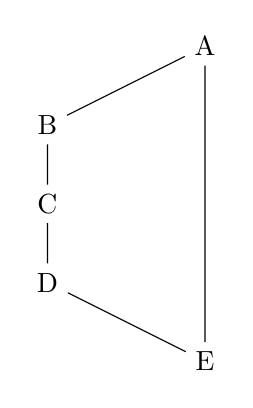
\begin{tikzpicture}
  \node (a) at (0,1) {A};
  \node (b) at (-2,0) {B};
  \node (c) at (-2,-1) {C};
  \node (d) at (-2,-2) {D};
  \node (e) at (0,-3) {E};
  \draw (e) -- (a) -- (b) -- (c) -- (d) -- (e);
\end{tikzpicture}
\end{center}
\endminipage
\minipage{0.50\textwidth}
\begin{center}
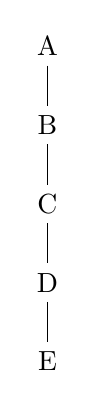
\begin{tikzpicture}
  \node (a) at (0,1) {A};
  \node (b) at (0,0) {B};
  \node (c) at (0,-1) {C};
  \node (d) at (0,-2) {D};
  \node (e) at (0,-3) {E};
  \draw (a) -- (b) -- (c) -- (d) -- (e);
\end{tikzpicture}
\end{center}
\endminipage

\subsection*{Příklad č.~8}

V Booleově algebře $(X, \oplus, \odot, {}^{\prime}, 0, 1)$ zjednodušte výrazy:

\begin{eqnarray*}
(a \oplus c) \oplus (c \oplus b) \oplus (b \oplus a) &=&
a \oplus a \oplus b \oplus b \oplus c \oplus c = \\ &=&
a \oplus b \oplus c
\end{eqnarray*}

\begin{eqnarray*}
(x \odot y) \oplus (x \odot z) \oplus (x^{\prime} \odot z^{\prime})^{\prime} &=&
(x \odot y) \oplus (x \odot z) \oplus (x \oplus z) = \\ &=&
[\lbrace x \odot (y \oplus z) \rbrace \oplus x] \oplus z = \\ &=&
[x \oplus x] \oplus z = \\ &=&
x \oplus z
\end{eqnarray*}

\begin{eqnarray*}
(x^{\prime} \oplus y^{\prime})^{\prime} &=&
x \odot y
\end{eqnarray*}

\newpage

\subsection*{Příklad č.~9}

Buď $G$ úplný graf o $n$ vrcholech. Určete počet cest délky 2, které začínají v pevně zvoleném vrcholu $a$ a končí v jiném pevně zvoleném vrcholu $b$. Kolik existuje takových cest délky 3? Zobecněte tento výsledek pro libovolné $k$, kde $1 \leq\ k < n$.

\minipage{0.8\textwidth}
\begin{tikzpicture}[->,>=stealth',level/.style={sibling distance = 5cm/#1,level distance = 1.5cm}]
\node (a) {A}
  child{
    node (a1) {1}
    child{
      node (a12) {2}
      child{ node (a123) {3}}
    }
    child{
      node (a13) {3}
	  child{ node (a132) {2}}
    }
  }
  child{
    node (a2) {2}
    child{
      node (a21) {1}
	  child{ node (a213) {3}}
    }
    child{
      node (a23) {3}
	  child{ node (a231) {1}}
    }
  }
  child{
    node (a3) {3}
    child{
      node (a31) {1}
	  child{ node (a312) {2}}
    }
    child{
      node (a32) {2}
	  child{ node (a321) {1}}
    }
  }
;
\node (b) at (0, -7) {B};
\draw (a123) -- (b);
\draw (a132) -- (b);
\draw (a213) -- (b);
\draw (a231) -- (b);
\draw (a312) -- (b);
\draw (a321) -- (b);
\end{tikzpicture}
\endminipage
\minipage{0.2\textwidth}
\begin{eqnarray*}
\frac{(n - 2)!}{(n - k - 1)!}
\end{eqnarray*}
\endminipage

Graf rozložíme na strom cest, které vedou z počátečního bodu (A) do koncového (B).
Pak počet cest vedoucí z každého dalšího uzlu je o 1 menší, než počet cest vedoucí z předchozího uzlu. Takže můžeme zapsat, že celkový počet cest vedoucí z uzlů je roven faktoriálu z celkového počtu uzlů bez dvou, počátečního a koncového.\\

Pokud chceme zjistit počet cest s určitou délkou, odebereme tu část faktoriálu kterou nepotřebujeme.\\

Tento vzorec můžeme zapsat jako:
\begin{eqnarray*}
\frac{(n - 2)!}{((n - 2) - (k - 1))!}
\end{eqnarray*}
kde $n$ je celkový počet uzlů a $k$ je počet hran v cestě.\\

Po zjednodušení dostaneme vzorec:
\begin{eqnarray*}
\frac{(n - 2)!}{(n - k - 1)!}
\end{eqnarray*}
\minipage{0.33\textwidth}
\printNgon{3}\\*
Počet vrcholů n = 3\\*
Počet cest délky k=2 je 1
\endminipage
\minipage{0.33\textwidth}
\printNgon{4}\\*
Počet vrcholů n = 4\\*
Počet cest délky k=2 je 2\\*
Počet cest délky k=3 je 2
\endminipage
\minipage{0.33\textwidth}
\printNgon{5}\\*
Počet vrcholů n = 5\\*
Počet cest délky k=2 je 3\\*
Počet cest délky k=3 je 6\\*
Počet cest délky k=4 je 6
\endminipage

\newpage

\subsection*{Příklad č.~10}

Nakreslete graf se šesti vrcholy, který lze nakreslit jedním uzavřeným tahem, ale v němž neexistuje hamiltonovská kružnice. Náležitě zdůvodněte, že tento graf má požadované vlastnosti. \\

\minipage{0.5\textwidth}
\begin{center}
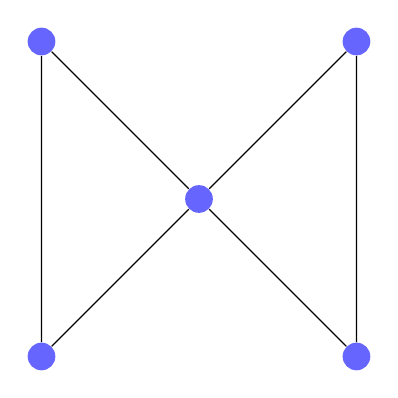
\begin{tikzpicture}[main_node/.style={circle,fill=blue!60,minimum size=1em,inner sep=3pt]}]
    \node[main_node] (1) at (-2, -2) {};
    \node[main_node] (2) at (-2, 2) {};
    \node[main_node] (3) at (0, 0) {};
    \node[main_node] (4) at (2, 2) {};
    \node[main_node] (5) at (2, -2) {};
    \draw (1) -- (2) -- (3) -- (4) -- (5) -- (3) -- (1);
\end{tikzpicture} \\
V grafu není hamiltonovská kružnice. \\
Cesta je uzavřená a prochází všemi vrcholy. \\
Nemá 6 vrcholů.
\end{center}
\endminipage
\minipage{0.5\textwidth}
\begin{center}
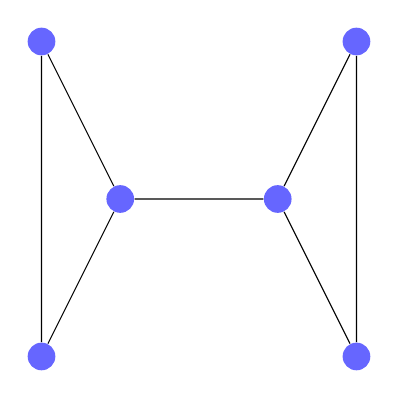
\begin{tikzpicture}[main_node/.style={circle,fill=blue!60,minimum size=1em,inner sep=3pt]}]
    \node[main_node] (1) at (-2, -2) {};
    \node[main_node] (2) at (-2, 2) {};
    \node[main_node] (3) at (-1, 0) {};
    \node[main_node] (4) at (1, 0) {};
    \node[main_node] (5) at (2, 2) {};
    \node[main_node] (6) at (2, -2) {};
    \draw (1) -- (2) -- (3) -- (4) -- (5) -- (6) -- (4) -- (3) -- (1);
\end{tikzpicture} \\
V grafu není hamiltonovská kružnice. \\
Nelze zakreslit jedním uzavřeným tahem. \\
Má 6 vrcholů.
\end{center}
\endminipage
\begin{center}
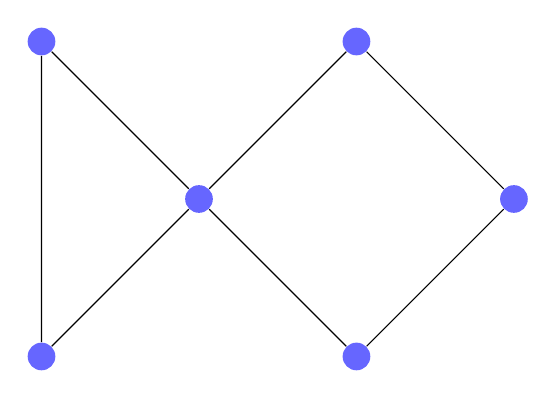
\begin{tikzpicture}[main_node/.style={circle,fill=blue!60,minimum size=1em,inner sep=3pt]}]
    \node[main_node] (1) at (-2, -2) {};
    \node[main_node] (2) at (-2, 2) {};
    \node[main_node] (3) at (0, 0) {};
    \node[main_node] (4) at (2, 2) {};
    \node[main_node] (5) at (4, 0) {};
    \node[main_node] (6) at (2, -2) {};
    \draw (1) -- (2) -- (3) -- (4) -- (5) -- (6) -- (3) -- (1);
\end{tikzpicture} \\
V grafu není hamiltonovská kružnice. \\
Cesta je uzavřená a prochází všemi vrcholy. \\
Má 6 vrcholů.
\end{center}
